\documentclass[a4paper]{article}

\usepackage{fullpage} % Package to use full page
\usepackage{parskip} % Package to tweak paragraph skipping
\usepackage{tikz} % Package for drawing
\usepackage{amsmath}
\usepackage{hyperref}
\usepackage[utf8]{inputenc}
\usepackage{lmodern}
\usepackage[MeX]{polski}
\usepackage[T1]{fontenc}
\usepackage{graphicx}
\usepackage{float}
\usepackage{subfiles}
\usepackage{booktabs}
\usepackage{multirow}
\usepackage{xparse}
\usepackage[most]{tcolorbox}
\usepackage{fancyvrb,newverbs,xcolor}

\definecolor{cverbbg}{gray}{0.93}

\newenvironment{lcverbatim}
{\SaveVerbatim{cverb}}
{\endSaveVerbatim
\flushleft\fboxrule=0pt\fboxsep=.5em
\colorbox{cverbbg}{%
\makebox[\dimexpr\linewidth-2\fboxsep][l]{\BUseVerbatim{cverb}}%
}
\endflushleft
}

\title{Notatki z kursu Bazy Danych 2}
\author{Małgorzata Dymek}
\date{2019/20, semestr zimowy}

\begin{document}
    \maketitle

    \section{Charakterystyki baz danych.}

    \subsection{Bazy danych produkcyjne}
    \begin{itemize}
        \item inaczej: \textbf{operacyjne}.
        \item wykorzystywana, gdy istnieje potrzeba nie tylko gromadzenia, ale też modyfikowania danych
        \item \textbf{dane dynamiczne}, tzn. ulegające zmianą i przedstawiające \textbf{aktualny stan rzeczy}
        \item \textbf{duża liczba prostych zapytań} od wielu użytkowników
        \item \textbf{zoptymalizowane} pod kątem \textbf{szybkiego wyszukiwania}
        \item np. baza inwentaryzacyjna, baza obsługi zamówień
    \end{itemize}


    \textbf{OLTP}
    \begin{itemize}
        \item \textbf{Online Transaction Processing}
        \item kategoria \textbf{aplikacji klient-serwer} dotyczących baz danych w ramach \textbf{bieżącego
        przetwarzania transakcji}
        \item klient współpracuje z \textbf{serwerem transakcji}, zamiast z serwerem bazy danych.
        \item np. systemy rezerwacji, obsługa punktów sprzedaży, systemy śledzące itp.
    \end{itemize}

    \subsection{Hurtownie danych}
    \begin{itemize}
        \item zorganizowana pod kątem pewnego \textbf{wycinka rzeczywistości} (tematycznie spójna)
        \item wyższy szczebel \textbf{abstrakcji} niż zwykła relacyjna baza danych
        \item dane często pochodzą z \textbf{wielu źródeł}
        \item \textbf{zoptymalizowabe} pod kątem \textbf{szybkości wyszukiwania} i \textbf{efektywnej analizy} zawartości.
        \item wyróżniany jest \textbf{poziom danych detalicznych} oraz \textbf{warstwa
        agregatów}/kostek tematycznych.
        \item korzystanie z danych hurtowni poprzez różne systemy
        wyszukiwania danych (np. OLAP).
        \item \textbf{brak} zastosowania typowych \textbf{transakcji}
        \item eksploracja danych (\textbf{data mining}) wyszukuje \textbf{ogólne formy wiedzy} z olbrzymiej ilości danych
        \item \textbf{wyszukiwania} mają najczęściej \textbf{charakter wielowymiarowy} – korzystają z wielu relacji.
        \item \textbf{tematycznie hurtownie} danych nazywane minihurtowniami danych (z ang. \textbf{data mart})
        \item \textbf{Cele} hurtowni
        \begin{table}[H]
            \begin{center}
                \begin{tabular}{p{7cm} p{9cm}}
                    \begin{itemize}
                        \item przetwarzanie analityczne (OLAP)
                        \item wspomaganie decyzji (DSS)
                        \item archiwizacja danych
                    \end{itemize}
                    &
                    \begin{itemize}
                        \item analiza efektywności
                        \item wsparcie dla systemów CRM (Customer Relationship Management)
                    \end{itemize}
                \end{tabular}
            \end{center}
        \end{table}
    \end{itemize}

    \begin{table}[H]
        \begin{center}
            \begin{tabular}{ |p{8cm}|p{8cm}| }
                \hline
                \multicolumn{2}{|c|}{\textbf{Data warehouse vs Data mart}}\\
                \hline
                \hline
                \textbf{Data warehouse} & \textbf{Data mart}\\
                \hline
                Dla całego przedsiębiorstwa & Dla konkretnego działu \\
                \hline
                Wiele obszarów tematycznych & Jeden konkretny obszar tematyczny \\
                \hline
                Trudna i czasochłonna do zbudowania & Łatwa i szybka do zbudowania \\
                \hline
                Duże zapotrzebowanie na pamięć & Małe zapotrzebowanie na pamięć \\
                \hline
            \end{tabular}
        \end{center}
    \end{table}

    Dwa \textbf{główne podejścia} wykorzystywane przy budowie hurtowni danych to:
    \begin{itemize}
        \item \textbf{ETL (Extract, Transform, Load)} - dane są wyciągane z różnych źródeł, następnie transformowane do formatu danych wymaganego przez hurtownie, a na końcu dopiero są ładowane do samej hurtowni
        \item \textbf{ELT (Extract, Load, Transform)} - dane są wyciągane z różnych źródeł, następnie ładowane od razu do hurtowni (do tabel roboczych) gdzie są dopiero transformowane i kopiowane do właściwych tabel hurtowni
    \end{itemize}

    \textbf{Architektura}
    \begin{itemize}
        \item \textbf{Źródło danych} – inne bazy danych (najcześciej relacyjne), różnego rodzaju pliki.
        \item \textbf{Obszar przejściowy} – dane pobrane z systemów źródłowych są oczyszczane i dostosowane do wymagań hurtowni danych (narzędzia ETL)
        \item \textbf{Warstwa metadanych}
        \begin{itemize}
            \item metadane \textbf{biznesowe}: tabele wymiarów, data marty, agregaty, tabele faktów
            \item metadane \textbf{techniczne}: mapowania i transformacje danych od systemu źródłowego do systemu docelowego
        \end{itemize}
        \item \textbf{Warstwa prezentacji} – warstwa dostępna dla użytkowników końcowych w postaci raportów i analiz; reprezentowana w postaci \textbf{data martów}
    \end{itemize}

    \subsubsection{Znormalizowane vs. wielowymiarowe podejście do gromadzenia danych}
    \textbf{Podejście wielowymiarowe} - model \textbf{gwiazdy}.
    \begin{itemize}
        \item transakcje danych są podzielone albo na poszczególne "fakty", które są generalnie transakcjami numerycznymi, albo "wielowymiarowe", które odnoszą się do kontekstów tych "faktów"
        \item \textbf{zaleta}: hurtownia danych jest prostsza do zrozumienia i użytkowania
        \item \textbf{wady}:
        \begin{itemize}
            \item skomplikowane utrzymanie porządku i integracji faktów wielowymiarowych
            \item trudno jest zmodyfikować hurtownię danych jeżeli przyjmuje się podejście wielowymiarowe zmieniając sposób
            organizacji danych.
        \end{itemize}
    \end{itemize}

    \textbf{Podejście znormalizowane} (model 3NF) - model \textbf{normalizacyjny} (E-R).
    \begin{itemize}
        \item tabele pogrupowane według ich \textbf{tematyki}
        \item dzieli dane na jednostki, które tworzą kilka tabel w relacyjnej
        bazie danych
        \item główną \textbf{zaletą} tego podejścia jest to, że \textbf{dodawanie} nowych informacji
        do bazy danych jest bardzo proste
        \item \textbf{wady}:
        \begin{itemize}
            \item ogromna ilość tabel
            \item łączenie danych z różnych źródeł w sensowne informacje jest trudne
            \item dostęp do danych wymaga precyzyjnego zrozumienia źródeł danych i ich struktur w hurtowni
        \end{itemize}
    \end{itemize}


    \subsection{Bazy analityczne: OLAP}
    \begin{itemize}
        \item \textbf{Kostki} OLAP (\textbf{Online Analytical Processing}), bazy analityczne (archiwalne)
        \item \textbf{dane} często pochodzą z bazy operacyjnej, ale po wprowadzeniu do bazy
        analitycznej są \textbf{stałe, nie podlegają modyfikacjom}
        \item główne operacje: \textbf{wyszukiwanie}, sporządzanie \textbf{zestawień statystycznych}, przeprowadzanie
        \textbf{analiz} i \textbf{prognoz}
        \item \textbf{niewielka liczba zapytań} dotycząca \textbf{dużych ilości danych}
        \item dane przechowywane w sposób przypominający \textbf{wielowymiarowe arkusze}; więcej biż trzy wymiary = \textbf{hiperkostka}
    \end{itemize}

    \subsubsection{Budowa kostki}
    \begin{itemize}
        \item \textbf{Fakty} - pojedyncze \textbf{zdarzenia}, które rejestrujemy (np. sprzedaż danego produktu)
        \begin{itemize}
            \item Każdy fakt ma \textbf{miary} - są to \textbf{wskaźniki numeryczne} związane z danym faktem (ile?)
            \item Oprócz miar w tabeli faktów są \textbf{klucze obce do wymiarów} opisujących dany fakt
        \end{itemize}
        \item \textbf{Wymiary} - \textbf{cechy} opisujące dany fakt (np. kto, co kiedy?) używane przy filtrowaniu
        \begin{itemize}
            \item Każdy wymiar ma \textbf{atrybuty} - są to po prostu \textbf{dane związane z} danym \textbf{wymiarem} (np. dla wymiaru daty sprzedaży będą to numer dnia, numer miesiąca i numer roku)
        \end{itemize}
    \end{itemize}

    \begin{table}[H]
        \begin{center}
            \begin{tabular}{p{8cm} p{8cm}}
                \multicolumn{2}{c}{\textbf{TYPOWE OPERACJE}}\\
                \begin{itemize}
                    \item \textbf{Zwijanie} – agregacja, uogólnienie danych,
                    \item \textbf{Rozwijanie} – uszczegółowienie danych,
                    \item \textbf{Selekcja} – wybór interesujących danych,
                    \item \textbf{Projekcja} – zmniejszenie liczby wymiarów,
                \end{itemize}
                &
                \begin{itemize}
                    \item \textbf{Wycinanie} – połączenie selekcji z projekcją,
                    \item \textbf{Sortowanie} – tworzenie rankingów,
                    \item \textbf{Obracanie} – zmiana perspektywy oglądania danych.
                \end{itemize}\\
            \end{tabular}
        \end{center}
    \end{table}

    \begin{table}[H]
        \begin{center}
            \begin{tabular}{p{8cm} p{8cm}}
                \multicolumn{2}{c}{\textbf{RODZAJE KOSTEK}}\\
                \textbf{fizyczne} & \textbf{wirtualne}\\
                posiadają w swoich komórkach już przeliczone i zagregowane dane
                &
                powstają z kostek fizycznych,

                mogą mieć swoje własne miary,

                wymiary dziedziczą po kostkach fizycznych
            \end{tabular}
        \end{center}
    \end{table}

    \begin{table}[H]
        \begin{center}
            \begin{tabular}{p{8cm} p{8cm}}
                \multicolumn{2}{c}{\textbf{SCHEMATY BUDOWY KOSTEK}}\\
                \textbf{gwiazda} & \textbf{płatek śniegu}\\
                \begin{itemize}
                    \item każda tabela wymiarów zawiera pełen zestaw atrybutów opisujących dany wymiar
                    \item może prowadzić do redundancji
                \end{itemize}
                &
                \begin{itemize}
                    \item każda tabela wymiarów zawiera tylko atrybuty specyficzne dla siebie
                    \item może też zawierać klucze obce do kolejnych tabel wymiarów
                \end{itemize}
            \end{tabular}
        \end{center}
    \end{table}

    \subsection{Jeziora danych}
    \begin{itemize}
        \item \textbf{ogromna ilość nieprzetworzonych danych w oryginalnym formacie} (strukturalne, częściowo lub zupełnie nie strukturalne)
        \item dane \textbf{łatwodostępne} i \textbf{modyfikowalne}
        \item każdy element znajdujący się w repozytorium ma przypisany
        \textbf{unikalny identyfikator} i jest oznaczany zestawem znaczników metadanych
        \item pozwala na maksymalnie szybką, zaawansowaną i kontekstową \textbf{analizę danych} nie tylko \textbf{historycznych}, ale
        także tych \textbf{generowanych} w czasie rzeczywistym
        \item dane mogą być np. wykorzystane do późniejszego zasilenia hurtowni danych lub w ogóle nie zostać nigdy użyte
        \item zazwyczaj wymagają zdecydowanie większej ilości \textbf{przestrzeni dyskowej} niż hurtownie danych
    \end{itemize}


    \subsection{Bazy danych NoSQL}
    \begin{itemize}
        \item \textbf{Not Only SQL}, non SQL, non relational
        \item łatwo \textbf{skalowalne horyzontalnie} (w klastrach i na wielu serwerach)
        \item przydatne w przypadku danych o \textbf{dużym wolumenie}
        \item celowo \textbf{rezygnuje się ze spójności} na rzecz większej wydajności i tolerancji na partycjonowanie
        \item nieunikanie \textbf{redundancji}, jest ona wręcz pożądana
        \item \textbf{główne typy}
        \begin{table}[H]
            \begin{center}
                \begin{tabular}{p{7cm} p{4cm} p{5cm}}
                    \begin{itemize}
                        \item Klucz-Wartość
                        \item Hierarchiczna struktura klucz-wartość
                    \end{itemize}
                    &
                    \begin{itemize}
                        \item Dokumentowe
                        \item Grafowe
                    \end{itemize}
                    &
                    \begin{itemize}
                        \item Kolumnowe
                    \end{itemize}
                \end{tabular}
            \end{center}
        \end{table}
        \item pozwalają na \textbf{szybką analizę} danych niestrukturyzowanych i badanie korelacji pomiędzy nimi
        \item \textbf{brak} łączenia (\textbf{JOIN}) danych po stronie serwera - jeżeli zachodzi taka potrzeba musi to być wykonywane po stronie aplikacji
        \item obiekty różnego typu: JSON, \textbf{BSON}, XML lub inny zbliżony, \textbf{przekazywane} są wraz \textbf{z
        kompletnym} ich \textbf{schematem}.
    \end{itemize}

    \begin{table}[H]
        \begin{center}
            \begin{tabular}{p{8cm} | p{8cm}}
                \textbf{ZALETY} & \textbf{WADY}\\
                \hline
                \begin{itemize}
                    \item są bardziej przystosowane i \textbf{wydajniejsze} przy przetwarzaniu \textbf{Big Data},
                    \item modele danych – \textbf{brak predefiniowanych schematów} powoduje ich większą \textbf{elastyczność},
                    \item potrafią przetwarzać \textbf{dane niestrukturalne},
                    \item \textbf{tańsze} i \textbf{prostsze} w utrzymaniu (szczególnie w przypadku prostych baz klucz-wartość),
                    \item z natury \textbf{skalowalne} (łatwe skalowanie horyzontalne).
                \end{itemize}
                &
                \begin{itemize}
                    \item dla danych, w których występują \textbf{relacje} zalecane są nadal standardowe RDBMS,
                    \item niemożność uniknięcia \textbf{redundancji},
                    \item mniejsza \textbf{integralność} i \textbf{spójność} danych,
                    \item SQL jest szeroko znany,
                    \item \textbf{brak mechanizmów transkacyjnych} – może nie spełniać zasady \textbf{ACID} (ang. Atomicity, Consistensy, Isolation, Durability)
                \end{itemize}\\
            \end{tabular}
        \end{center}
    \end{table}

    \subsection{Big Data}
    \begin{itemize}
        \item duże, zmienne i różnorodne \textbf{zbiory danych}, których przetwarzanie i analiza jest trudna
        \item dwie główne grupy:
        \begin{itemize}
            \item \textbf{Ustrukturyzowane} - najczęściej dane wewnętrzne firmy (np. dane ze stacji pogodowych)
            \item \textbf{Nieustrukturyzowane} - najczęściej dane pobierane z portali społecznościowych lub ogólniej Internetu
        \end{itemize}
        \item ponieważ zapytania muszą być wykonywane szybko, wszystkie \textbf{analizy} wykonuje się \textbf{równolegle}
    \end{itemize}

    Trzy \textbf{podstawowe cechy} (\textbf{3xV}):
    \begin{itemize}
        \item \textbf{Volume} (amount) of data - duża ilość danych
        \item \textbf{Velocity} (speed) of collecting - są one gromadzone z ogromną szybkością
        \item \textbf{Variety} of info - duża różnorodność gromadzonych danych
    \end{itemize}

    Najpopularniejszymi \textbf{narzędziami} do pomiaru Big Data są:
    \begin{table}[H]
        \begin{center}
            \begin{tabular}{p{5cm} p{10cm}}
                \begin{itemize}
                    \item platforma \textbf{Hadoop},
                    \item system Storm,
                \end{itemize}
                &
                \begin{itemize}
                    \item \textbf{magazyny baz} danych – Cassandra, MongoDB czy Neo4j,
                    \item algorytmy do \textbf{data-miningu} – RapidMiner i Mahout,
                \end{itemize}
            \end{tabular}
        \end{center}
    \end{table}

    \section{Poziomy izolacji transkacji.}
    \textbf{Problemy:}
    \begin{itemize}
        \item \textbf{P0 (Dirty Write)}: $T_1$ modyfikuje daną. $T_2$ modyfikuje tą samą daną zanim $T_1$ zostanie zaakceptowana (lub anulowana).
        \item \textbf{A1 (Dirty Read)}: $T_1$ modyfikuje daną. $T_2$ czyta daną zanim $T_1$ zostaje zaakceptowana. Jeżeli $T_1$ zostanie wycofana, $T_2$ ma odczyt danej która "nigdy nie istniała".
        \item \textbf{A2 (Non-repeatable or Fuzzy Read)}: $T_1$ czyta daną. Następnie $T_2$ modyfikuje albo usuwa tą daną i zostaje zatwierdzona. Gdy $T_1$ próbuje powtórzyć odczyt, dostaje inną wartość albo okazuje się, że dana została usunięta.
        \item \textbf{A3 (Phantom)}: $T_1$ odczytuje zestaw danych zaspokajających klauzulę WHERE. Następnie $T_2$ dodaje rekordy które spełniają tą klauzulę i zostaje zaakceptowana. GDY $T_1$ próbuje powtórzyć odczyt dostaje inny zestaw danych.
        \item \textbf{P4 Lost update}: $T_1$ odczytuje daną i wylicza nową wartość. $T_2$ odczytuje daną i wylicza nową wartość. $T_1$ zapisuje wartość i zostaje zaakceptowana, $T_2$ nadpisuje tą wartość i zostaje zaakceptowana.
    \end{itemize}

    A - oryginalna definicja, P - rozszerzona.\\

    P0: w1[x]...w2[x]...((c1 lub a1) i (c2 lub a2) w dowolnej kolejności)\\

    A1: w1[x]...r2[x]...(a1 i c2 w dowolnej kolejności)\\
    P1: w1[x]...r2[x]...((c1 lub a1) i (c2 lub a2) w dowolnej kolejności)\\

    A2: r1[x]...w2[x]...c2...r1[x]...c1\\
    P2: r1[x]...w2[x]...((c1 lub a1) i (c2 lub a2) w dowolnej kolejności)\\

    A3: r1[P]...w2[y in P]...c2...r1[P]...c1\\
    P3: r1[P]...w2[y in P]...((c1 lub a1) i (c2 lub a2) w dowolnej kolejności)\\

    P4: r1[x]...w2[x]…c2 ...w1[x]...c1\\\\

    \begin{tabular}{|c||c|c|c|c|}
        \hline
        \textbf{Poziom izolacji} & \textbf{P0} Dirty Write & \textbf{P1} Dirty Read & \textbf{P2} Non-repeatable/Fuzzy Read & \textbf{P3} Phantoms \\
        \hline
        \hline
        \textbf{READ UNCOMMITED} & NIE & TAK & TAK & TAK \\
        \hline
        \textbf{READ COMMITED} & NIE & NIE & TAK & TAK \\
        \hline
        \textbf{REPEATABLE READ} & NIE & NIE & NIE & TAK\\
        \hline
        \textbf{SERIAZABLE} & NIE & NIE & NIE & NIE\\
        \hline
    \end{tabular}

    \subsection{Izolacja dla systemów z blokowaniem}
    \textbf{Blokada} (lock) jest \textbf{zmienną związaną z elementem danych}, która opisuje \textbf{stan} tego elementu
    pod względem \textbf{możliwości działań}, jakie mogą być na nim w danej chwili wykonywane.\\

    \textbf{Dobrze sformowane zapisy} - przed zapisem \textbf{wymagane jest założenie blokady X} (ew. predykatowej).\\
    \textbf{Dobrze sformowane odczyty} - do operacji odczytu \textbf{wymagane jest założenie blokady S} (ew. predykatowej).\\

    \textbf{Blokada U} - gdy element danych \textbf{jest odczytywany i być może będzie potem aktualizowany}.
    Podnoszenie S na X moze prowadzić do \textbf{zakleszczenia}. Jest zakładana \textbf{przy odczycie}, przed wykonaniem
    aktualizacji \textbf{jest konwertowana do X}.\\

    \begin{tabular}{|c||c|c|c|}
        \hline
        \textbf{przyznana} v / \textbf{przyznawana} $\rightarrow$ & \textbf{S} & \textbf{X} & \textbf{U} \\
        \hline
        \hline
        \textbf{S} & tak & nie & tak\\
        \hline
        \textbf{X} & nie & nie & nie\\
        \hline
        \textbf{U} & tak/nie & nie & nie\\
        \hline
    \end{tabular}

    \subsubsection{Podstawowe poziomy izolacji}
    \begin{tabular}{|c||c|c|c|c|c|c| }
        \hline
        \textbf{Poziom izolacji} & \textbf{P0} & \textbf{P1} & \textbf{P2} & \textbf{P3} & Blokady \textbf{X} & Blokady \textbf{S} \\
        \hline
        \hline
        \textbf{Locking READ UNCOMMITED} & NIE & TAK & TAK & TAK & długie & nie \\
        \hline
        \textbf{Locking READ COMMITED} & NIE & NIE & TAK & TAK & długie & krótkie\\
        \hline
        \textbf{Locking REPEATABLE READ} & NIE & NIE & NIE & TAK & długie & długie\\
        \hline
        \textbf{Locking SERIAZABLE} & NIE & NIE & NIE & NIE & długie & długie predykatowe\\
        \hline
    \end{tabular}

    \subsubsection{Poziom izolacji Cursor Stability}
    \textbf{Rozszerzenie} sposobu blokowania w poziomie \textbf{Locking READ COMMITTED}. Dodaje się \textbf{operację
    rc (czytaj kursor, pobierz wiersz)} dla instrukcji \textbf{FETCH}, blokada (\textbf{S} lub nowy typ blokady do
    dczytu \textbf{scroll lock}) będzie utrzymywana \textbf{do chwili przejścia} do innego wiersza lub do
    \textbf{zamknięcia} kursora.\\

    \textbf{Aktualizacja wiersza przez kursor} – operacja \textbf{wc} powoduje założenie na ten wiersz \textbf{długiej blokady X}.\\

    Dla operacji na kursorze można zdefiniować odmianę problemu \textbf{P4 Lost Update}:\\
    \textbf{P4C: rc1[x]...w2[x]...c2...wc1[x]...c1}\\

    Poziom izolacji Cursor Stability \textbf{eliminuje P4C}, w2[x] będzie wstrzymane do zdjęcia blokady (S, scroll lock) przez przejście do innego wiersza lub zamknięcie kursora.\\
    Uwaga: READ COMMITTED << Cursor Stability << REPEATABLE READ

    \subsection{Poziom izolacji Snapshot i podobne}
    Transakcja czyta dane (zatwierdzone) z \textbf{chwili swojego
    początku}, Start-Timestamp. \\

    \begin{itemize}
        \item \textbf{Snapshot isolation (MS SQL Server SNAPSHOT)}
        \begin{itemize}
            \item Są stosowane \textbf{blokady do zapisu}, ponadto przy każdym zapisie transakcja wykonuje podobne sprawdzenie jak wykonywane w propozycji 1 na końcu transakcji.
            \item Przechowywane są \textbf{różne wersje danych}. Transakcja \textbf{odczytuje dane aktualne} w momencie rozpoczęcia transakcji.
            \item \textbf{Nie ma blokad do odczytu}, operacja odczytu nie blokuje operacji zapisu ani innych operacji odczytu. Są jednak stosowane \textbf{długie blokady wyłączne do zapisu}.
            \item Transakcja $T_1$ przy każdym zapisie sprawdza, czy istnieje inna transakcja $T_2$, która zmodyfikowała dane zapisywane i zakończyła się zatwierdzeniem. Jeśli istnieje, to $T_1$ jest wycofywana.
            \item Stosowaną tu zasadę można określić jako \textbf{First-writer-wins}.
        \end{itemize}
        \item \textbf{Read Committed Snapshot (Oralce READ COMMITTED)}
        \begin{itemize}
            \item Oeracja odczytu \textbf{czyta ostatnią zatwierdzoną wartość} elementu danych (niekoniecznie sprzed początku transakcji).
            \item W przyjętej implementacji wiersze kursora czytane są w momencie otwarcia kursora, a nie w momencie odczytu wiersza.
        \end{itemize}
    \end{itemize}

    Poziom izolacji Snapshot \textbf{nie gwarantuje szeregowalności konfliktowej} harmonogramów.\\

    \textbf{A5 Data Item Constraint Violation}
    Załóżmy, że na elementy danych x oraz y narzucono pewne \textbf{ograniczenie C()}. Każda transakcja z osobna dba o spełnienie C().\\

    \textbf{A5A Skrzywiony odczyt (Read Skew)}\\
    $T_1$ odczytuje x, potem inna transakcja $T_2$ aktualizuje x
    oraz y do nowych wartości i zostaje zatwierdzona. Jeśli następnie $T_1$ odczyta y, to będzie miała niespójny obraz danych.\\
    \textbf{A5A: r1[x]...w2[x]...w2[y]...c2...r1[y]...(c1 or a1)}\\

    \textbf{A5B Skrzywiony zapis (Write Skew)}\\
    $T_1$ odczytuje x (ew. odczytuje też y). Następnie inna
    transakcja $T_2$ odczytuje y (ew. odczytuje też x). Następnie $T_1$ zapisuje y a $T_2$ zapisuje x i
    obydwie zostają zatwierdzone. Ostatnie cztery operacje mogą być zrealizowane w dowolnej (sensownej) kolejności. Każda transakcja przy zapisie dba o spełnienie ograniczenia C(),
    jednak w wyniku przeplatanego wykonania ograniczenie C() może nie być spełnione po zatwierdzeniu obydwu transakcji.\\
    \textbf{A5B: r1[x]...r2[y]...(w1[y] w2[x] c1 i c2 w dowolnej sensownej kolejności)}\\

    \textbf{A5A oraz A5B nie wystąpią w harmonogramach, w których wykluczony jest P2.}\\

    \begin{tabular}{|c|c|c|c|c|c|c|}
        \hline
        & P0 & P1 & A3 & P3 & A5A & A5B \\
        \hline
        Snapshot Isolation & nie & nie & nie & tak & nie & tak\\
        \hline
        Read Commited & & & & & tak & \\
        \hline
        Locking Repeatable Read & & & & tak & & nie\\
        \hline
    \end{tabular}

    REPEATABLE READ >><< Snapshot Isolation


    \section{Kursory.}
    \begin{itemize}
        \item zmienne umożliwiające \textbf{sekwencyjny dostęp} do tabel
        \item pobranie wiersza: FETCH, zamknięcie kursosa: CLOSE, zwolnienie pamięci: DEALLOCATE
    \end{itemize}

    \subsection{ISO}:
    \begin{itemize}
        \item \textbf{INSENSITIVE} – tworzona jest kopia statyczna danych w bazie tempdb. Nie można aktualizować.
        \item \textbf{SCROLL} – można wykorzystywać wszystkie opcje FETCH: FIRST, LAST, PRIOR, NEXT, RELATIVE, ABSOLUTE (domyślnie można używać tylko NEXT).
        \item \textbf{READ ONLY} – nie można wykonywać \textbf{pozycjonowanych zmian danych} (np. UPDATE \dots WHERE CURRENT OF nazwakursora).
        \item \textbf{UPDATE OF} – można aktualizować \textbf{tylko wymienione kolumny} (samo UPDATE oznacza zgodę na aktualizacje wszystkich kolumn).
    \end{itemize}

    \subsection{T-SQL}:
    \begin{itemize}
        \item \textbf{LOCAL} – zakres (scope) kursora jest lokalny do wsadu (batch), procedury składowanej, wyzwalacza, gdzie kursor
        został zadeklarowany.
        \item \textbf{GLOBAL} – kursor będzie globalny dla
        połączenia. Zwolnienie pamięci będzie zrealizowane przy zamknięciu połączenia lub wskutek jawnie wykonanej operacji
        deallocate.
        \item \textbf{FORWARD\_ONLY} – określa, że kursor może być skrolowany tylko \textbf{od pierwszego do ostatniego wiersza} (można
        używać tylko FETCH NEXT).
        \begin{itemize}
            \item Jeśli nie wyspecyfikowano ani FORWARD\_ONLY ani SCROLL, ani STATIC/KEYSET/DYNAMIC, FORWARD\_ONLY jest przyjmowany
            \item Dla kursorów STATIC, KEYSET
            i DYNAMIC domyślną opcją jest SCROLL.
        \end{itemize}
        \item \textbf{STATIC} – odpowiednik \textbf{INSENSITIVE}.
        \item \textbf{KEYSET} – w bazie temdb tworzona jest tabela z wartościami klucza (kluczy) określającymi zestaw wierszy.
        \begin{itemize}
            \item Jeśli w chociaż jednej tabeli, do której odwołuje się kursor, nie ma indeksu unikalnego, to typ kursora zmieniany jest na
            STATIC.
            \item Zmiany na danych są widoczne poprzez kursor (w kolejnych operacjach FETCH), z wyjątkiem dodania nowego
            wiersza, skasowania wiersza lub aktualizacji klucza. Przy próbie pobrania nieistniejącego wiersza funkcja
            @@FETCH\_STATUS zwraca wartość -2.
        \end{itemize}
        \item \textbf{READ\_ONLY} – zmiany pozycjonowane nie są możliwe (domyślnie są).
        \item \textbf{OPTIMISTIC} – zmiany pozycjonowane są możliwe, jest realizowane optymistyczne sterowanie współbieżnością.
        \item \textbf{SCROLL LOCK} – zmiany pozycjonowane są możliwe, jest realizowane pesymistyczne sterowanie współbieżnością z blokadami.
        \begin{itemize}
            \item Jeśli nie wyspecyfikowano ani READ\_ONLY, ani OPTIMISTIC ani SCROLL LOCK, to będzie przyjęte ustawienie według poniższych reguł:
            \begin{itemize}
                \item Jeśli zdanie SELECT nie wspiera aktualizacji (np. niewystarczające uprawnienia), kursor
                będzie READ\_ONLY.
                \item Standardowo kursory STATIC i FAST\_FORWARD są READ\_ONLY.
                \item Standardem dla kursorów DYNAMIC i KEYSET jest OPTIMISTIC.
            \end{itemize}
        \end{itemize}
    \end{itemize}

    \subsection{Sterowanie współbieżnością}
    \begin{itemize}
        \item \textbf{OPTIMISTIC WITH VALUES} - na początku wczytujemy wartości w wierszach, przed zapisaniem sprawdzamy
        czy się nie zmieniły
        \item \textbf{OPTIMISTIC WITH ROW VERSIONS} - mamy dodatkową kolumnę row version, którą sprawdzamy by się upewnić
        że nie było zmian
        \item \textbf{SCROLL\_LOCKS (pesimistic)} - zakładamy blokadę = gwarancja sukcesunaszej operacji
    \end{itemize}

    \subsection{Przykład}
    Np. kiedy chcemy utworzyć logi kto co usunął - trigger dla usuwania i zapisanie poszczególnych wierszy wraz z user id
    do tabeli logów.

    \section{Obsługa transakcji w procedurach składowanych.}
    \begin{lcverbatim}
        CREATE PROC [dbo].[usp_my_proc] (@arg1 INT, @arg2 VARCHAR(25))
        AS
        DECLARE @tran_count AS INT
        SET @tran_count = @@TRANCOUNT

        IF @tran_count > 0
        SAVE TRAN save_point
        ELSE
        BEGIN TRAN

        BEGIN TRY

        -- SQL code goes here

        IF @tran_count > 0
        COMMIT TRAN save_point
        ELSE
        COMMIT
        END TRY
        BEGIN CATCH
        IF @tran_count > 0
        ROLLBACK TRAN save_point
        ELSE
        ROLLBACK
        END CATCH;
        GO
    \end{lcverbatim}


    \section{Odtwarzanie baz danych po awarii.}
    \textbf{LSN} - log sequence number.

    \textbf{Checkpoint} - moment \textbf{zrzucenia buforowanych} w pamięci logów transakcji i stron (\textbf{dirty
    pages}) na dysk oraz ustawienia LSN checkpointu w boot page.

    \textbf{Transaction logs} są \textbf{obcinane} w momencie checkpointu (przeważnie \textbf{automatycznie co} pewien
    \textbf{określony czas}). W zależności od ustawionego \textbf{recovery model}:
    \begin{itemize}
        \item \textbf{Simple Recovery Model} - transaction logs są \textbf{ucinane do momentu rozpoczęcia pierwszej niezatwierdzonej transakcji}. Serwer w razie awarii może:
        \begin{itemize}
            \item \textbf{automatycznie przywrócić niezsynchronizowane} jeszcze z plikiem strony \textbf{dane},
            \item \textbf{wycofać} te, które \textbf{nie} zostały \textbf{zatwierdzone} a są już \textbf{zapisane} do pliku strony.
        \end{itemize}
        \item \textbf{Full or Bulk-Logged Recovery Models} - transaction logs są \textbf{ucinane do momentu ostatniej kopii zapasowej} tych logów. Możliwe jest:
        \begin{itemize}
            \item odtworzenie stanu danych aż do momentu samej awarii (w Simple Recovery Model jedynie do momentu ostatniej pełnej lub różnicowej kopii, ponieważ potem nie mamy logów).
        \end{itemize}
    \end{itemize}


    \subsection{Przywracanie bazy danych po awarii dysków (plików z danymi)}
    \textbf{Zakładamy tu, że pliki z logami przetrwały!}

    \begin{enumerate}
        \item Tworzymy \textbf{kopię zapasową logów} transakcji, które nie zostały zbackupowane wcześniej
        \begin{lcverbatim}
            BACKUP LOG <database_name> TO <backup_device>
            WITH NORECOVERY, NO_TRUNCATE;
        \end{lcverbatim}
        \item Odtwarzamy \textbf{pełną kopię zapasową}
        \begin{lcverbatim}
            RESTORE DATABASE <database_name> FROM <backup_device>
            WITH NORECOVERY;
        \end{lcverbatim}
        \item (Ewentualnie) Odtwarzamy \textbf{kopię różnicową} wykonaną po kopii pełnej z poprzedniego punktu
        \begin{lcverbatim}
            RESTORE DATABASE <database_name> FROM <backup_device>
            WITH NORECOVERY;
        \end{lcverbatim}
        \item \textbf{Aplikujemy każdy zbackupowany} transaction \textbf{log} (włącznie z tym zbackupowanym na samym początku) zawierający logi od ostatniej odtworzonej kopii zapasowej
        \begin{lcverbatim}
            RESTORE LOG <database_name> FROM <backup_device>
            WITH NORECOVERY;
        \end{lcverbatim}
        \item Na końcu wydajemy \textbf{komendę} mówiącą bazie danych, że \textbf{odtwarzanie zostało} już \textbf{ukończone} i baza danych może być normalnie używana
        \begin{lcverbatim}
            RESTORE DATABASE <database_name>
            WITH RECOVERY;
        \end{lcverbatim}
    \end{enumerate}

    \textbf{Podczas procesu} odtwarzania z opcją \textbf{NORECOVERY baza} danych \textbf{nie} jest normalnie
    \textbf{dostępna} (nie możemy z niej korzystać). Ponadto:
    \begin{itemize}
        \item Operacje ``\textbf{roll back}'' \textbf{nie} są jeszcze \textbf{wykonywane}.
        \item Operacje ``\textbf{roll forward}'' się \textbf{wykonują}.
        \item Umożliwia nam to zaaplikowanie kolejnego logu transakcji czy backupu.
        \item Dopiero
        podczas aplikowania \textbf{ostatniego logu} transakcji możemy dać opcję \textbf{WITH RECOVERY} co spowoduje \textbf{wykonanie} wszystkich
        operacji ``\textbf{roll back}'' i uznanie tej\textbf{bazy} danych za \textbf{w pełni odtworzoną}, a przez to \textbf{dostępną} już normalnie dla
        wszystkich użytkowników.
    \end{itemize}

    Ustawienie opcji \textbf{WITH STANDBY} pozwala (administratorom) \textbf{wykonywać odczyty} na tej bazie danych. Wymaga
    podajania ścieżki do \textbf{pliku standby} (zostanie utworzony).

    \section{Mirroring i database snapshot.}
    \subsection{Mirroring}
    \begin{itemize}
        \item Zazwyczaj jest zestawiany \textbf{między odległymi} od siebie \textbf{maszynami}
        \item Mirroring odbywa się \textbf{na poziome baz} danych a \textbf{nie} całego \textbf{serwera}
        \item Aby baza danych mogła być mirrorowana \textbf{na obu serwerach musi być} ustawiony dla tej bazy danych \textbf{full recovery model}
        \begin{itemize}
            \item \textbf{mirroring opiera się na przesyłaniu logów} transakcji pomiędzy serwerami
        \end{itemize}
        \item Jest tylko \textbf{jeden principale} i \textbf{jeden mirror} oraz opcjonalnie \textbf{jeden witness} (przynajmniej w MSSQL serverze):
        \begin{itemize}
            \item \textbf{Principale} - jest to \textbf{serwer produkcyjny}. Udostępnia on swoją bazę do odczytu i zapisu.
            \item \textbf{Mirror} - jest to serwer, który utrzymuje \textbf{kopię danych} z principala aby móc w razie potrzeby przejąć jego rolę. Dane na tym serwerze nie są dostępne ani do odczytu, ani do zapisu.
            \item \textbf{Witness} - jest to serwer, który \textbf{nie przechowuje} żadnych \textbf{danych}, a jedynie \textbf{utrzymuje kontakt} z principalem i mirrorem.
            \item \textbf{Automatic failover}
            Jeśli:
            \begin{itemize}
                \item mirror nie ma kontaktu z principalem,
                \item mirror ma kontakt z witnessem,
                \item witness również stracił kontakt z principalem
            \end{itemize}
            Wtedy uznaje się \textbf{principala za niedostępnego i mirror staje się principalem}. Aby automatic failover działał, \textbf{mirroring} musi być skonfigurowany w trybie \textbf{high-safety}
        \end{itemize}
        \item Mirroring może być skonfigurowany w dwóch trybach:
        \begin{itemize}
            \item \textbf{High-safety mode (synchroniczny)} - w tym trybie aby \textbf{transakcja} przeprowadzana \textbf{na principale} mogła zostać uznana za \textbf{zatwierdzoną}, principal musi poczekać na \textbf{potwierdzenie od mirrora} odnośnie wpisania danych związanych z tą transakcją do jego dziennika transakcji.
            \item \textbf{High-performance (asynchroniczny)} - w tym trybie aby \textbf{transakcja na principalu} została \textbf{zatwierdzona nie musi on czekać} na potwierdzenie od mirrora. \textbf{Dane do mirrora} odnośnie wykonanych operacji są \textbf{wysyłane niezależnie} (jak najszybciej).
        \end{itemize}
        \item \textbf{Połączenie między serwerami} może być \textbf{zabezpieczane} przy pomocy \textbf{Windows authentication} albo \textbf{Certificate-based authentication}.
    \end{itemize}

    \subsection{Database snapshot}
    \begin{itemize}
        \item Snapshot jest pełnym obrazem bazy danych z momentu jego utworzenia
        \item Dostępny tylko do odczytu
        \item Używa mechanizmu ``copy-on-write'', co w tym przypadku oznacza, że tylko strony danych, które zostały zmienione od czasu utworzenia snapshotu są kopiowane do specjalnych plików (sparse files). Z tego wynika że w najgorszym przypadku utrzymywanie snapshotu może zająć dodatkowo tyle miejsca na dysku ile zajmowała oryginalna baza danych w momencie jego tworzenia.
        \item Zastosowania:
        \begin{itemize}
            \item Posiadanie stanu danych z pewnego okresu, np. w celu utworzenia raportu
            \item Swego rodzaju zabezpieczenie przed utratą danych na wypadek błędu po stronie administratora lub użytkownika - ze snapshotu można zawsze przekopiować z powrotem dane do właściwej bazy danych lub przywrócić ją w prost ze snapshota przy użyciu komendy RESTORE DATABASE. Snapshoty \textbf{nie zastępują jednak kopii zapasowych}, ponieważ nie można na przykład odtworzyć z nich uszkodzonej bazy danych lub bazy, która jest offline
            \item Trzymanie szeregu snapshotów z różnych okresów czasu może być używane do analizy zmian jakie zaszły w tych danych
        \end{itemize}
        \item Tworzenie snapshotu:
        \begin{lcverbatim}
            CREATE DATABASE <database_snapshot_name>
            ON (NAME = <logical_file_name>, FILENAME = <file_path>)
            AS SNAPSHOT OF <source_database_name>
        \end{lcverbatim}
    \end{itemize}


    \section{Replikacja.}
    \begin{center}
        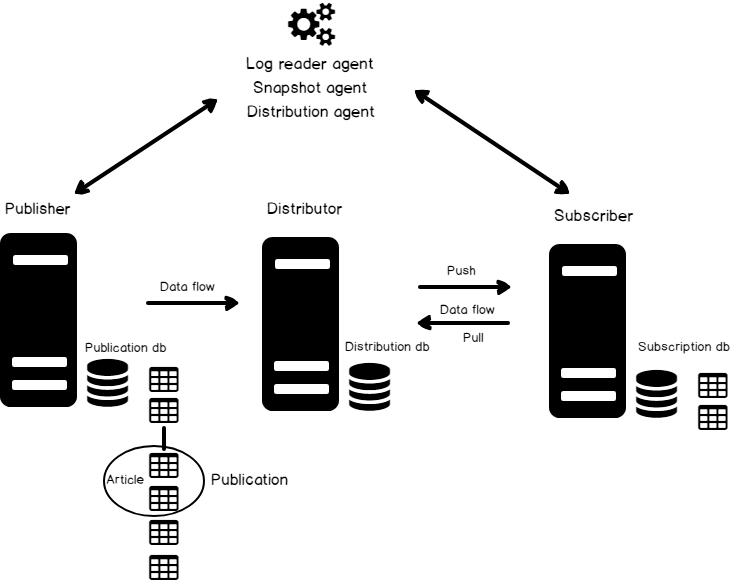
\includegraphics[width=\textwidth]{replication}
    \end{center}

    \subsection{Definicja}
    Replikacja to proces powielania informacji pomiędzy różnymi serwerami baz danych. Ze wszystkich kopii można korzystać,
    w przeciwieństwie do mirroringu.

    \begin{itemize}
        \item \textbf{Article} - \textbf{obiekt} bazy danych (tabela, procedura składowana, itp.), który jest \textbf{opublikowany} (będzie dostępny dla Subscriberów)
        \item \textbf{Publication} - \textbf{logiczna kolekcja} opublikowanych \textbf{obiektów} (Articlów) umożliwiająca również \textbf{konfigurację} ich \textbf{atrybutów} (np. co ma się stać gdy dana tabela lub procedura składowana już istnieje w docelowej bazie danych)
        \item \textbf{Publisher} - \textbf{baza} danych \textbf{zawierająca publikowane} zasoby
        \item \textbf{Distributor} - \textbf{pośrednik} w \textbf{wymianie danych} między Publisherem a Subscribentem. \textbf{Przechowuje metadane} odnośnie publikacji, w niektórych konfiguracjach jest także \textbf{buforem} dla przekazywanych danych. Na dystrybutorze mamy co najmniej jedną \textbf{Distribution database}, która przechowuje wspomniane metadane. Każdy Publisher ma swoją Distribution database na dystrybutorze.
        \item \textbf{Subscriber} - \textbf{instancja bazy} danych, która \textbf{pobiera dane} od Publishera. Subscriber może pobierać dane \textbf{z wielu publikacji}. W zależności od konfiguracji może również \textbf{przekazywać} te dane do innych baz (działać jako Publisher), lub \textbf{odsyłać modyfikacje} przeprowadzone po jego stronie na synchronizowanych danych z powrotem do Publishera
        \item \textbf{Subscribtion database} - \textbf{docelowa baza} danych dla replikowanych obiektów
    \end{itemize}


    \subsection{Podstawowe metody replikacji w systemie Microsoft SQL Server}

    Najważniejsze \textbf{typy publikacji}:
    \begin{itemize}
        \item \textbf{Snapshot publication} - jest to \textbf{jednorazowy transfer} z Publishera do Subskrybenta. \textbf{Po dokonaniu} tego \textbf{transferu} danych żadne \textbf{zmiany} wykonane po którejkolwiek ze stron \textbf{nie są} dalej \textbf{śledzone}.
        \item \textbf{Transactional publication} - umożliwia \textbf{prawie natychmiastowe aktualizowanie danych} zmienionych na Publisherze do Subscribenta. \textbf{Przeważnie} i domyślnie jest to \textbf{replikacja tylko w jedną stronę}, aczkolwiek istnieje możliwość obustronnego jej skonfigurowania.\\
        \textbf{Dwa główne sposoby} aktualizowania zmienionych danych:
        \begin{itemize}
            \item \textbf{Push} - \textbf{Distributor} bezpośrednio \textbf{aktualizuje} dane na subskrybencie. Wtedy Distribution Agent działa na Distributorze i ``wypycha'' dane do Subscribenta
            \item \textbf{Pull} - \textbf{Subskrybent} sam co jakiś czas \textbf{pobiera} zmodyfikowane dane z Distributora. W tym przypadku Distribution Agent działa na Subscribencie i ``zaciąga'' dane z Distributora (na dystrybutorze musi być \textbf{udostępniony udział Windows} z danymi do pobrania - przez to ze względu na uwierzytelnienie, dostępne jest to tylko w domenie Windows?)
        \end{itemize}
        \item \textbf{Peer-to-peer replication} - w tym typie replikacji \textbf{zmiany mogą być wprowadzane na każdej z baz} danych.
        \begin{itemize}
            \item Baza na której została wprowadzona zmiana wysyła ją jak najszybciej do pozostałych tak aby wszystkie z nich miały spójną kopię.
            \item \textbf{Mogą wystąpić niespójności danych} w przypadku, gdy ta sama porcja danych zostanie w tym samym czasie zmodyfikowana na wielu węzłach.
            \item Niespójności muszą być \textbf{rozwiązywane ręcznie}. (?)
        \end{itemize}
        \item \textbf{Merge replication} - ten tryb zakłada \textbf{synchronizację danych} z pozostałymi węzłami \textbf{co określony czas}.
        \begin{itemize}
            \item W momencie synchronizacji danych \textbf{zmiany} są \textbf{mergowane}, a ewentualne konflikty (automatycznie?) rozwiązywane.
            \item Węzły \textbf{nie muszą być cały czas podłączone} do sieci.
            \item \textbf{Łączność} sieciowa z Distribiutorem jest \textbf{wymagana} tylko \textbf{w momencie synchronizacji} danych.
        \end{itemize}
    \end{itemize}

    \section{Widoki rozproszone.}

    \section{Podstawowa charakterystyka transakcji rozproszonych.}

    Transakcja rozproszona to transakcja, której polecenia DML (insert, update, delete) i select odwołują się do tabel
    znajdujących się co najmniej w dwóch węzłach rozproszonej bazy danych. Transakcja rozproszona jest często nazywana
    transakcją globalną.


    \section{MongoDB.}
    \begin{itemize}
        \item \textbf{otwarty, nierelacyjny} system zarządzania bazą danych
        \item duża \textbf{skalowalność} i \textbf{wydajność}
        \item \textbf{brak ściśle zdefiniowanej struktury} obsługiwanych baz danych
        \item dane składowane są jako \textbf{dokumenty JSON}, co umożliwia aplikacjom bardziej naturalne ich przetwarzanie zachowując
        możliwości tworzenia \textbf{hierarchii} oraz \textbf{indeksowania}.
        \item dokumenty umieszczone są w \textbf{kolekcjach} przechowywanych w bazach danych
        \item \textbf{model działania:}
        \begin{itemize}
            \item model asynchronicznych zapisów i eventual consistency,
            \item klient otrzymuje jedynie obietnicę, że dane zostaną zapisane w przyszłości
        \end{itemize}
        \item \textbf{możliwości}:
        \begin{itemize}
            \item jednorodne wsparcie dla standardu Unicode,
            \item obsługa danych w innych kodowaniach w formacie binarnym,
            \item duża liczba obsługiwanych typów danych,
            \item obsługa kursorów,
            \item zapytania ad-hoc,
            \item zapytania do zagnieżdżonych pól dokumentów,
            \item indeksowanie,
            \item wsparcie dla agregacji danych,
            \item możliwość składowania plików w bazie,
            \item architektura zaprojektowana z myślą o łatwej replikacji,
            \item łatwa skalowalność,
            \item brak joinów,
            \item brak ograniczenia schematami danych
        \end{itemize}
        \item wewnętrznym językiem do definiowania zapytań oraz funkcji agregujących jest JavaScript wykonywany bezpośrednio przez serwer MongoDB.
        \item \textbf{wady:}
        \begin{itemize}
            \item w domyślnych ustawieniach bazy MongoDB dostępne są \textbf{publicznie}, bez hasła.
            \item problemy ze spójnością danych wynikające z błędów implementacyjnych modelu (naprawione),
            \item problemy z kompletnością zwracanych dokumentów przy wyszukiwaniach z użyciem indeksów (pomijanie aktualnie aktualizowanych)
            \item ograniczone wsparcie kodowania UTF-8
        \end{itemize}
    \end{itemize}

    \subsection{Podstawowe operacje}
    \subsubsection{Insert}
    \begin{lcverbatim}
        >db.COLLECTION_NAME.insert(document)
    \end{lcverbatim}
    Jeśli nie wyspecyfikujemy \_id w dokumencie, MongoDB wygeneruje dla niego unikalny identyfikator.

    Analogicznie działa metoda save(), jednak dla wyspecyfikowanego \_id może podmienić dane na nowe (insert wyrzuci błąd).

    \subsubsection{Find}
    \begin{lcverbatim}
        >db.COLLECTION_NAME.find(query)
    \end{lcverbatim}
    Wykonuje kwerendę na kolekcji, zwraca dokumenty w sposób nieustrukturyzowany (można je sformatować używając pretty()).

    Wywołany \textbf{bez argumentu} zwraca \textbf{wszystkie} dokumenty w kolekcji. Argumentem jest \textbf{kwerenda}:
    \begin{table}[H]
        \begin{center}
            \begin{tabular}{| p{0.5cm} || p{4cm} | p{6cm} | p{4.5cm} |}
                \hline
                \textbf{Op} & \textbf{Syntax} & \textbf{Example} & \textbf{RDBMS Equivalent}\\
                \hline
                \hline
                $==$ & \{<key>:<value>\} & db.mycol.find(\{"by":"tutorials point"\}) & where by = 'tutorials point'\\
                \hline
                $<$ & \{<key>:\{\$lt:<value>\}\} & db.mycol.find(\{"likes":\{\$lt:50\}\}) & where likes < 50\\
                \hline
                $\leq$ & \{<key>:\{\$lte:<value>\}\} & db.mycol.find(\{"likes":\{\$lte:50\}\}) & where likes <= 50\\
                \hline
                $>$ & \{<key>:\{\$gt:<value>\}\} & db.mycol.find(\{"likes":\{\$gt:50\}\}) & where likes > 50\\
                \hline
                $\geq$ & \{<key>:\{\$gte:<value>\}\} & db.mycol.find(\{"likes":\{\$gte:50\}\}) & where likes >= 50\\
                \hline
                $\neq$ & \{<key>:\{\$ne:<value>\}\} & db.mycol.find(\{"likes":\{\$ne:50\}\}) & where likes != 50\\
                \hline
            \end{tabular}
        \end{center}
    \end{table}

    Można używać również \textbf{AND} jako db.mycol.find(\{\$and: [ \{key1: value1\}, \{key2: value2\}]\}) lub po prostu db.mycol.find(\{\{key1: value1\}, \{key2: value2\}\}).

    \textbf{OR} analogicznie: db.mycol.find(\{\$or: [ \{key1: value1\}, \{key2: value2\}]\}).
    \
    \section{XML w systemie Microsoft SQL Server.}


    \begin{itemize}
        \item W SQL Serverze 2000 dodano klauzulę \textbf{FOR XML}, która pozwala zwrócić wynik kwerendy jako XML. \textbf{AUTO} zapisuje informacje jako atrybuty, dodanie \textbf{ELEMENTS} - jako podelementy.
        \item W SQL Serverze 2005 dodano \textbf{typ danych XML}. Pozwala on natywnie \textbf{przechowywać} dokumenty i fragmenty XML \textbf{w kolumnach i zmiennych}.
        \item Typ danych XML zapewnia \textbf{odpowiednie formatowanie} danyych, tj. \textbf{zgodne} ze \textbf{standardami ISO}.
        \item Obiekty typu XML mają narzucone pewne \textbf{ograniczenia}:
        \begin{itemize}
            \item Instancja XML nie może przekroczyć \textbf{2GB}.
            \item Kolumna typu XML \textbf{nie} może być \textbf{kluczem głównym} tabeli.
            \item \textbf{Nie} można używać obiektów XML w klauzuli \textbf{GROUP BY}.
            \item \textbf{Nie} można \textbf{porównywać} ani \textbf{sortować} danych typu XML.
        \end{itemize}
        \item Użycie typu XML nie zawsze jest \textbf{potrzebne} - jeśli zamierzamy je tylko przechować, bez przeszukiwania czy zmieniania, można użyć np. VARCHAR(MAX). Unikniemy w ten sposób wywoływania parsera, który jest obciążający obliczeniowo.
        \item \textbf{Schemat kolekcji XML} (XML schema collection) składa się z jednego lub więcej \textbf{schematów definicji XML} (XML Schema Definition, XSD), używanych do walidacji danych znajdujących się w obiekcie XML. Zawierają faktyczne formatowanie informacji, definiują ich strukturę i typy danych; na jego podstawie jest parsowany XML.
        \item SQL Server rozróżnia \textbf{dokumenty i fragmenty} XML. Jeśli obiekt XML jest typowany, to można określić czy przyjmuje oba, czy tylko pełne dokumnety.
        \item Metoda \textbf{query()} zwraca \textbf{instancję} nietypowanego XMLa będącą \textbf{podzbiorem} większego obiektu.
        \item Metoda \textbf{value()} zwraca \textbf{element} lub \textbf{wartość argumentu} (typ danych, nie fragment XML).
        \item Metoda \textbf{exist() testuje istnienie} elementu podanego argumentem. Zwraca:
        \begin{itemize}
            \item \textbf{1 (BIT)} jeśli element szukany \textbf{istnieje},
            \item \textbf{0 (BIT)} jeśli element szukany \textbf{nie istnieje},
            \item \textbf{NULL} jeśli XML podany do przeszukania jest \textbf{nullem}.
        \end{itemize}
        \item Metoda \textbf{nodes()} zwraca \textbf{tabelę} (wiersze) z pojedynczą kolumną, gdzie każdy wiersz zawiera pojedynczą instancję XMLa z wyniku zapytania. Używany w celu \textbf{podzielenia instancji} XMLa na \textbf{relacyjne dane}.
        \item Metoda \textbf{modify()} jest jedyną metodą pozwalającą \textbf{modyfikować} dane typu XML. Bierze jako argument wyrażenie w XML Data Modification Language (XML DML). Pozwala \textbf{wstawiać} (insert), \textbf{edytować} (replace) i \textbf{usuwać} (delete) dane w obiekcie XML.
    \end{itemize}


    \section{Przetwarzanie grafów ?.}

\end{document}
